% ----------------------------------------------------------------------------------
% A LIST OF EXPERIMENTS TO DO 
% ----------------------------------------------------------------------------------
\section{Experiments}
Notes about some experiments to do.

\begin{enumerate}

\item Calculate total schedulable time in a night and advance demand profiles.

Search p2db for any groups which are enabled that night and sum up total exec times. If they are monitors we need to add n times exec (for n windows). If flexible we should count seperately or maybe add in a fractional contribution for 1/(length (nights) of flex span). Similar for ephem groups. Do this for a year or semester - note the flex stuff becomes a bit weird as some would have been done do we want to deplete them as if actually done (P(done before tonight) = (t-flexstart)/span or the likes). want to normalize results by length of night (sus-sur or twi-twi). As weel as semesterly would be good to get this information as a profile for individual nights and showing subscription(t), priority(t) etc.

This is an indicator of over/under subscription. If we are undersubscribed any night we should be able to accomodate everything with a bit of negotiation /sliding. If oversubscribed then need to prioritize - e.g. auction prices set by demand ! The oversubscription rate is a useful piece of info to give PDAs - lets them know how bad competition is without divulging sensitive information from other PDAs. Also could allow view of profiles over the night of PDA requests by priority level. 

Scenario: start of night, SE asks PDAs to make reservations (not really just what i would like to get and what priority or \emph{score} is assigned  - by PDA or normallized? - no commitment but expect truthful!). SE makes profiles available to all PDAs. This sort of thing would let a PDA see if there were quiet or low priority slots available again without divulging too much information - any sort of statistical info like this is potentialy useful in decision making for bidding. 


\item Monte-carlo simulation to find range of scores using simple scheduling algorithm(s).

Step thro night, pick a group from feasibles (random selection), if none timestep a minute or so else time step exec time, repeat.
Count up total used time. count sum priorities, count cumulative score via various metrics.

Repeat this umpteen times to get ranges, mean and stds for these parameters and measuring score metrics using various parameterisations.

Want to see the range of schedules we could get to set some bounds on these. We would expect a real scheduler to do better than the worst case and hopefully as good as best case. We wont see the best case unless we do zillions of runs but may get some idea how far into the tail it is..

\item Various contention measures

\begin{itemize}
\item True contention over night as profile
\item Daily groups enabled in night at some point count over period of weeks/months
\item Daily groups enabled over night as profile
\item weighted contention profile
\item Probabilistic true contention as profile over night with different seeing assumptions -i.e. different curves and then various probabilty assumption curves plus a combined probabilty curve, maybe some envelopes.
\end{itemize}


\item Some notes about the simulation framework.

Need a framework to run the scheduler in. Currently looking at running scheduling engine continuously at some predefined rate with additional planning layers running at slower rate - how the Scheduler's run-rate (better name?) is chosen is dependant on the rate at which the ODB changes - if we run every 30 minutes and ODB changes \emph{significantly} on that timescale we will either miss opportunities or do unnecessary (unprofitable) work - both lead to reduced cumulative reward. Consequently the need for some sort of feedback from the ODB (Phase2Model) may be needed - suggests some sort of {\tt Phase2ModelUpdateListener} interface that the SE can register as. This would most likely just have a simple implementation like a method {\tt phase2ModelUpdated(Phase2Event pe)}. 

How do we decide when a \emph{significant} change has occurred ? -  Suggest each event type has some sort of weighting associated and we just increment a score as the events come in - maybe need to consider if the event's target is involved in the current schedule as part of the assessment. When a threshhold is exceeded this could prompt a rerun of the scheduler. We dont want the scheduler re-running each time an ODB change occurs - this will lead to reduced \emph{effective horizon} and reduced profit. Opportunity here for some learning - i.e. measure the rate of change of the ODB and set the scheduler run rate dependant on this - {\bf adaptive run rate} (better acronym please).

Because the (simulation) scheduler will be running faster than realtime (i.e. it will execute in realtime but gaps will be speeded up) and the executor (simulator) will also be running (in parallel) in model-time we need some way to synchronize the two - this suggests the need for a discrete event queue to control the model clock (i.e. {\tt DiscreteEventSimulationTimeModel}. This had {\bf not} previously been considered neccessary as the scheduler was expected to run on request from the Executor. This turns out to be a bit of a bugger to implement - not difficult for a simulated SE and Executor but I am exepecting to use the \emph{real} SE here. I would expect to have it run using some sort of polling loop i.e. something like:-

\begin{algorithm}
\While{true}{
 run scheduler\;
 sleep $\delta$ t\;
}
\caption{Realtime scheduler run cycle}
\end{algorithm}

To allow the \emph{real} SE to be used in simulation, in addition to being able to switch the {\tt TimeModel} from {\tt RealTimeModel} to {\tt SimulatedTimeModel} which can be set by the franework, it will be neccessary to privide simulated clock to inject events/triggers into the SE. I envisage something like:-

\begin{algorithm}
\While{true}{
 run scheduler\;
 wait on time signal {bf E} at $\delta$t\;
}
\caption{Simulation scheduler run cycle}
\end{algorithm}

To implement the line \emph{wait on time signal {\bf E} at $\delta$t},  The event/trigger {\bf E} - some class implementing {\tt EventObject} is something the scheduler would register with an {\tt EventGenerator} using the {\tt registerEvent(Event e, EventHandler h, long deltaTime}. In this case the {\tt EventHandler} is some object the SE would nominate to handle the return event from the {\tt EventGenerator} $\delta$T later. The SE would at this point do a wait on the handler. On completion of the wait, the SE continues execution - in effect this is just a round-about way of doing a sleep. Could allow various types of event and SE (or any other type of handler) could act on these appropriately but this is not really neccessary. The simulation framework would also need to make use of the {\tt EventGenerator} to register execution times of groups effectively being submitted to executor. 


   \begin{figure}[htp]
   \begin{center}
   \includegraphics[height=6cm]{figures/sim_framework.eps}
   \end{center}
   \label{fig:simframewrk} 
   \caption[Scheduling simulation framework.] 
   {Architecture of scheduling simulation framework.}
   \end{figure} 

Whats going on here ? The sim controller provides all the models for the SE - The EnvModel is likely generated on-the-fly based on current time and some provided function (or e.g. random variation about some mean level or with some trend...). The ExecModel likely uses a random variation


\item Some details about a test of different bias functions.

\item Effect of snapshot age on calculations - especially wrt (Problem Quality Metrics) PQMs.

What are the effects of various simulation assumptions ? Namely effects like phase2 drift. I will run a series of experments to test the effect of length of lookahead - this can be done using the following method:-
work out demand profile d(t) for N nights ahead. Run simulation for 1 night and recalculate - now for N-1 nights ahead, keep doing this so on step r we simulate night r and work out d(t) for N-r nights ahead. Variation on this could include the effects of varying the Env model. Basically I just want to know if look ahead calculation of D(t) works - can also compare this to working out D(t) for r using different ODB snapshots.


\end{enumerate}

\subsection{Investigation of database characteristics}

This is just a look at snapshots of the deployed ODB and various generated datasets to determine general characteristics and limits. A useful test is to examine the contention profile generated by various models by perfoming an overnight simulation - this differs from the prior contention profile which does not take into account those observations performed earlier in the night.

A set of standard execution models was generated:-

\begin{table}[h]
\begin{center}
\begin{tabular}{lllllll}
\toprule
\multicolumn{5}{c}{Standard Execution Models} \\
\midrule
Name & Offset(s) & Readout(s) & Slew(s) & Config(s) & MaxT(H) & Horizon($^{\circ}$) \\
\midrule
$X_{n/S}$      & 10     & 12      & 60   & 6  &  2  & 20 \\
$X_{n/L}$      & 10     & 12      & 60   & 6  &  4  & 20 \\
$X_{n/L/hi}$   & 10     & 12      & 60   & 6  &  4  & 30 \\
$X_{f/S}$      & 5      & 6       & 45   & 4  &  2  & 20 \\
$X_{f/L}$      & 5      & 6       & 45   & 4  &  4  & 20 \\
$X_{f/L/hi}$   & 5      & 6       & 45   & 4  &  4  & 30 \\
$X_{s/S}$      & 12     & 16      & 90   & 12 &  2  & 20 \\ 
$X_{s/L}$      & 12     & 16      & 90   & 12 &  4  & 20 \\ 
$X_{s/L/hi}$   & 12     & 16      & 90   & 12 &  4  & 30 \\ 
\bottomrule
\end{tabular}
\end{center}
\caption{Set of standard execution models. Classified as \emph{slow} (s), \emph{normal} (n) and \emph{fast} (f), with maximum execution times \emph{short} (S) and \emph{long} (L). \emph{Hi} models have extra high horizon. Additional models defined based on thes ebut with e.g. MaxT 30 minutes and horizon elevation 35$^{\circ}$ would be specified as $X_{n/30m/35d}$. }
\end{table}

Description of various characterisation simulations.
\begin{itemize}
\item demand profiles/load stats (all available snapshot nights using DC and LC.) -- dont diplay all these as latex will thorw a wobbly, jsut a selection for now.
\item Demand and load averages and min/max plot over whole season along with nightlength, moondark/astronight plots. Figure \ref{fig:cd_av_trend} shows the trend of $C_D$ over the available set of ODB snapshots.


\item run BST for a selection of nights multiple times to get contention (ensemble) plots over nights under efx,efp and several e-scenarios (make sure these are tabulated seperately).
\end{itemize}

\begin{figure}[h]
\begin{center}
 \subfigure[Trend of average value of demand profile $C_D$ for available ODB dataset]{
   \includegraphics[scale=0.25, angle=-90]{figures/cdtrend.eps}
   \label{fig:cd_av_trend}
 }
 \subfigure[Trend of peak value of demand profile $C_D$ for available ODB dataset]{
   \includegraphics[scale=0.25, angle=-90]{figures/cdmax.eps}
   \label{fig:cd_max_trend}
 }
\caption{Trends of demand statistics over available ODB snapshots}
\end{center}
\end{figure}


\subsection{Case Study 1}
This investigation involves running a series of one-night simulations under different environmental assumptions to see the effect of varying the value of the SHM weights $w_{trans}$ relative to the priority weight $w_p$.
The rational behind this investigation is to provide some initial insight into the usefulness of the various SQMs and to provide a shakedown test of the simulation framework on real data. By selecting 2 seperate but similar nights it should be possible to get a preliminary idea on the range of likely values fand variation of SQMs.


 The set of \emph{remaining} objective function weights ${W_x}$ excluding $w_{trans}$ and $w_p$ are kept constant at zero level throughout the range of test values to avoid any additional biasing. The SQMs used to evaluate the quality of the resulting schedules are $Q_{OA}$ - the optimal airmass metric, $Q_{PX}$ - the execution time weighted priority metric, $Q_{RN}$ - urgency metric, $Q_{TD}$ - demand metric, $Q_{PX \cdot OA}$ - priority weighted optimal airmass and $Q_X$ the total execution time as a fraction of available night. 

Two nights were considered. Both were similar in terms of amount of dark moon time though the actual night lengths were significantly different. Night 1, 13th-14th October 2007 has xxx hours of lunar dark time out of xxx hours night of which xxx hours are astronomicaly dark. Night 2, 7th-8th November 2007 has xxx hours of lunar dark time out of xxx hours night of which xxx hours are astronomicaly dark.


\begin{table}
\begin{center}
\caption{Case study night characteristics}
\begin{tabular}{lll}
\toprule
\multicolumn{2}{c}{Case study night characteristics} \\
\midrule
Item & Night 1 & Night 2 \\
\midrule
Date                & 14-15 Oct 2007 & 7-8 Nov 2007\\
Sunset              & 18:40          & 18:20\\
Sunrise             & 07:08          & 07:23\\
Start Astro night   & 19:58          & 19:40\\
End Astro night     & 05:50          & 06:03\\
Moonset             & 10:01          & 16:47\\
Moonrise            & 20:27          & 06:05\\
\midrule
Length of night     & 12:28          & 13:03\\
Length astro night  & 9:52           & 10:23\\
Length astro moon dark    & 7:23     & 10:03\\
Lunar dark fraction & 75\%           & 96.7\%\\
\bottomrule
\end{tabular}
\end{center}
\end{table}

A series of simulations were performed to determine the range of contention statistics for the 2 study nights. Figures \ref{fig:cont4_ensemble} and \ref{fig:cont6_ensemble} show ensemble results from a large number of simulations for the 2 nights.d \ref{fig:bsa1_ex}.

\begin{figure}[h]
 \begin{center}
  \subfigure[Contention profile $C_c$ ensemble for night 2.] {
    \label{fig:cont4_ensemble}
    \includegraphics[scale=0.25, angle=-90]{figures/cont4_ensemble.eps}
  }
  \subfigure[Contention profile $C_c$ ensemble for night 1.] {
    \label{fig:cont6_ensemble}
    \includegraphics[scale=0.25, angle=-90]{figures/cont6_ensemble.eps}
  }
\caption{Contention profile ensembles for case study nights 1 and 2} 
 \end{center}
\end{figure}

A comparison for several runs using fixed execution models and various environmental models are displayed in figures \ref{fig:bsa0_pr} and \ref{fig:bsa0_pr} (Wrong labels !)

\begin{figure}[h]
 \begin{center}
 \subfigure[Variation of contention profile $C_c$ under $E_{FP}$ night 1.] {
   \label{fig:bsa0_pr}
   \includegraphics[scale=0.25, angle=-90]{figures/bsa_pr_cont.eps}
  }
 \subfigure[Variation of contention profile $C_c$ under $E_{FX}$ night 1.] {
   \label{fig:bsa1_ex}
   \includegraphics[scale=0.25, angle=-90]{figures/bsa_ex_cont.eps}
  } 
  
  \subfigure[Variation of contention profile $C_c$ under $E_{RA}$ night 1.] {
   \label{fig:bsa2_rnd}
   \includegraphics[scale=0.25, angle=-90]{figures/bsa_rnd1_cont.eps}
  }
  \subfigure[Variation of contention profile $C_c$ under $E_{RA}$ night 1.] {
   \label{fig:bsa2_rnd}
   \includegraphics[scale=0.25, angle=-90]{figures/bsa_rnd2_cont.eps}
  } 

   \subfigure[Variation of contention profile $C_c$ under mixed environment for night 1.] {
   \label{fig:bsa2_rnd}
   \includegraphics[scale=0.25, angle=-90]{figures/bsa_combine_cont.eps}
  }
  \caption{Effects of environment model on contention profile for night 1}
 \end{center}
\end{figure}

\begin{figure}[h]
 \begin{center}
 \subfigure[Variation of contention profile $C_c$ under $E_{FP}$ night 2.] {
   \label{fig:bsa0_pr}
   \includegraphics[scale=0.25, angle=-90]{figures/bsb_pr_cont.eps}
  }
 \subfigure[Variation of contention profile $C_c$ under $E_{FX}$ night 2.] {
   \label{fig:bsa1_ex}
   \includegraphics[scale=0.25, angle=-90]{figures/bsb_ex_cont.eps}
  }
  
  \subfigure[Variation of contention profile $C_c$ under $E_{RA}$ night 2.] {
   \label{fig:bsa2_rnd}
   \includegraphics[scale=0.25, angle=-90]{figures/bsb_rnd1_cont.eps}
  }
  \subfigure[Variation of contention profile $C_c$ under $E_{RA}$ night 2.] {
   \label{fig:bsa2_rnd}
   \includegraphics[scale=0.25, angle=-90]{figures/bsb_rnd2_cont.eps}
  } 

   \subfigure[Variation of contention profile $C_c$ under mixed environment for night 2.] {
   \label{fig:bsa2_rnd}
   \includegraphics[scale=0.25, angle=-90]{figures/bsb_combine_cont.eps}
  }
 \caption{Effects of environment model on contention profile for night 2}
  
 \end{center}
\end{figure}


For both nights simulations were run using a basic rank scoring selection mechanism $\mathcal{S}_{BEST}$ which selects the highest scoring group from the set of candidate metrics. In addition a second simulation was performed using a random selection model $\mathcal{S}_{Random}$ in which all candidates have equal chance of selection irrespective of their relative scores. This was to provide an indication of how well the normal selection and scoring mechanisms perform against a baseline.

The following models were fixed in all cases:-
\begin{itemize}
 \item Charge Accounting Model $\mathcal{C}$ is described in \ref{tab:cam_param}.
 \item Scoring model $\mathcal{S}$ was setup initially with no weighting parameters as these are to be varied during the experment.
 \item Execution timing and feasibility model $X$ is described in \ref{tab:etm_param}.
 \item Stochastic execution mode $\mathcal{\zeta}$ is described in \ref{tab:sex_param}.
\end{itemize}

\clearpage
\begin{landscape}
\begin{table}
\begin{center}
\caption{Fixed model parameters for all simulations}
\centering
\subtable[Charge accounting model parameters. These are used to work out the accounting debit on completion of a group execution]{
\label{tab:cam_param}
\begin{tabular}{ll}
\toprule
\multicolumn{2}{c}{Charge Accounting Model} \\
\midrule
Accounting parameter & Value(sec) \\
\midrule
Offset & 10\\
Slewing rotation & 60 \\
Instrument configuration & 5 \\
Instrument readout & 12\\
\bottomrule
\end{tabular}
}
\subtable[Execution timing and feasibility  model parameters. These are used to determine whether a group can execute at a given time under specified environmental conditions and with given execution history and to \emph{estimate} how long it is likely to take]{
\label{tab:etm_param}
\begin{tabular}{lll}
\toprule
\multicolumn{3}{c}{Execution Feasibility and Timing Model} \\
\midrule
Execution model parameter & Value & Units \\
\midrule
Dome horizon & 20 & $^{\circ}$\\
Dome zenith limit & 89 & $^{\circ}$ \\
Solar night elevation & -18 & $^{\circ}$ \\
Dark twilight elevation & -12.0 & $^{\circ}$\\
Bright twilight elevation & -6.0  & $^{\circ}$\\
Fixed group pre-start buffer & 200 & sec\\
Fixed group post-start lapse & 900 & sec\\
Max execution time & 7200 & sec\\
Offset & 10 & sec\\
Slewing rotation & 60 & sec \\
Instrument configuration & 6 &sec \\
Instrument readout & 12 & sec\\
\bottomrule
\end{tabular}
}
\subtable[Lost the description]{
\label{tab:sex_param}
\begin{tabular}{lll}
\toprule
\multicolumn{3}{c}{Stochastic Execution Timing  Model} \\
\midrule
Execution timing parameter & Minimum value (sec) & Maximum value (sec) \\
\midrule
Offset & 5 & 12\\
Slewing rotation & 30 & 120 \\
Instrument configuration & 6 & 12 \\
Instrument readout & 8 & 13\\
\bottomrule
\end{tabular}     
}
\end{center}
\end{table}
\end{landscape}

Results of the random selection models were as follows:-

\begin{table}
\begin{center}
\begin{tabular}{lllllll}
\toprule
\multicolumn{7}{c}{Results for Random slection model $\zeta_{random}$} \\
\midrule
 & $Q_{OA}$ & $Q_{PX}$ & $Q_{TD}$ & $Q_{X}$ & $Q_{RN}$ & $Q_{PX\cdotOA}$\\ 
\midrule
{\bf Average} & 0.835  & 1.332  & 2.957  & 0.907  & 23.976 & 1.086\\
{\bf Minimum} & 0.775  & 0.921  & 1.417  & 0.881  & 15.331 & 0.765\\
{\bf Maximum} & 0.887  & 1.698  & 5.000  & 0.932  & 33.225 & 1.417\\
{\bf SDev}    & 0.0225 & 0.1357 & 0.8021 & 0.0081 & 3.6253 & 0.1258\\
\bottomrule
\end{tabular}
\end{center}
\end{table}

First results revealed a surprisingly minor effect of varying $w_{trans}$ especially at values of $w_{trans}$ from 0 to 50\% where the plot is particularly flat. The plot then rises rapidly at some cut-in point - further investigation is suggested to see if the cut-in point depends on environment and load factors. In addition the non-linear domain sampling suggested the need for a different regime of domain sampling. 


\clearpage
\begin{figure}[h]
 \begin{center}
  \subfigure[Effect of varying $w_{trans}$ relative to $w_{p}$ on $Q_{PX}$ schedule quality metric]{
    \label{fig:cs1_dw1_px}
    \includegraphics[scale=0.25, angle=-90]{figures/cs1_dw1_px.eps}
  }
  \subfigure[Effect of varying $w_{trans}$ relative to $w_{p}$ on $Q_{OA}$ schedule quality metric]{
    \label{fig:cs1_dw1_oa}
    \includegraphics[scale=0.25, angle=-90]{figures/cs1_dw1_oa.eps}
  }
  \subfigure[Effect of varying $w_{trans}$ relative to $w_{p}$ on $Q_{OA}$ schedule quality metric for Flexible groups]{
    \label{fig:cs1_dw1_foa}
    \includegraphics[scale=0.25, angle=-90]{figures/cs1_dw1_foa.eps}
  }
  \subfigure[Effect of varying $w_{trans}$ relative to $w_{p}$ on $Q_{PX}$ schedule quality metric for Flexible groups]{
    \label{fig:cs1_dw1_fpx}
    \includegraphics[scale=0.25, angle=-90]{figures/cs1_dw1_fpx.eps}
  }
  \subfigure[Effect of varying $w_{trans}$ relative to $w_{p}$ on $Q_{TD}$ schedule quality metric]{
    \label{fig:cs1_dw1_td}
    \includegraphics[scale=0.25, angle=-90]{figures/cs1_dw1_td.eps}
  }
  \subfigure[Effect of varying $w_{trans}$ relative to $w_{p}$ on $Q_{RN}$ schedule quality metric]{
    \label{fig:cs1_dw1_rn}
    \includegraphics[scale=0.25, angle=-90]{figures/cs1_dw1_rn.eps}
  }
\caption{Results for night 2 (7-8 November 2007) for environment model $E_{FP}$} 
 \end{center}
\end{figure}


\clearpage
\begin{figure}[h]
 \begin{center}
  \subfigure[Effect of varying $w_{trans}$ relative to $w_{p}$ on $Q_{PX}$ schedule quality metric]{
    \label{fig:cs1_dw1_px}
    \includegraphics[scale=0.25, angle=-90]{figures/cs1_dw2_px.eps}
  }
  \subfigure[Effect of varying $w_{trans}$ relative to $w_{p}$ on $Q_{OA}$ schedule quality metric]{
    \label{fig:cs1_dw1_oa}
    \includegraphics[scale=0.25, angle=-90]{figures/cs1_dw2_oa.eps}
  }
  \subfigure[Effect of varying $w_{trans}$ relative to $w_{p}$ on $Q_{OA}$ schedule quality metric for Flexible groups]{
    \label{fig:cs1_dw1_foa}
    \includegraphics[scale=0.25, angle=-90]{figures/cs1_dw2_foa.eps}
  }
  \subfigure[Effect of varying $w_{trans}$ relative to $w_{p}$ on $Q_{PX}$ schedule quality metric for Flexible groups]{
    \label{fig:cs1_dw1_fpx}
    \includegraphics[scale=0.25, angle=-90]{figures/cs1_dw2_fpx.eps}
  }
  \subfigure[Effect of varying $w_{trans}$ relative to $w_{p}$ on $Q_{TD}$ schedule quality metric]{
    \label{fig:cs1_dw1_td}
    \includegraphics[scale=0.25, angle=-90]{figures/cs1_dw2_td.eps}
  }
  \subfigure[Effect of varying $w_{trans}$ relative to $w_{p}$ on $Q_{RN}$ schedule quality metric]{
    \label{fig:cs1_dw1_rn}
    \includegraphics[scale=0.25, angle=-90]{figures/cs1_dw2_rn.eps}
  }
\caption{Results for night 2 (7-8 November 2007) for environment model $E_{FX}$} 
 \end{center}
\end{figure}
 
\clearpage
% comparison graphs
\begin{figure}[h]
\begin{center}
  \subfigure[Comparison of effect of environment model ($E_{FP}$, $E_{FX}$) on $Q_{OA}$ for variable $w_{trans}$.]{
   \includegraphics[scale=0.25, angle=-90]{figures/cs1_dw1a2_oa.eps}
   \label{fig:cs1_dw1a2_oa}
  }
  \subfigure[Comparison of effect of environment model ($E_{FP}$, $E_{FX}$) on $Q_{PX}$ for variable $w_{trans}$.] {
    \includegraphics[scale=0.25, angle=-90]{figures/cs1_dw1a2_px.eps}
    \label{fig:cs1_dw1a2_px}
  }
  \subfigure[Comparison of effect of environment model ($E_{FP}$, $E_{FX}$) on $Q_{RN}$ for variable $w_{trans}$.] {
    \includegraphics[scale=0.25, angle=-90]{figures/cs1_dw1a2_rn.eps}
     \label{fig:cs1_dw1a2_rn}
  }
  \subfigure[Comparison of effect of environment model ($E_{FP}$, $E_{FX}$) on $Q_{TD}$ for variable $w_{trans}$.] {
    \includegraphics[scale=0.25, angle=-90]{figures/cs1_dw1a2_td.eps}
    \label{fig:cs1_dw1a2_td}
  }
  \subfigure[Comparison of dependancy of $Q_{OA}$ on $w_{trans}$ for all groups and flexible groups under environment model $E_{FP}$.]{
    \includegraphics[scale=0.25, angle=-90]{figures/cs1_dw1_oa_c.eps}
    \label{fig:cs1_dw1_oa_c}
  }
  \subfigure[Comparison of dependancy of $Q_{PX}$ on $w_{trans}$ for all groups and flexible groups under environment model $E_{FP}$.]{
    \includegraphics[scale=0.25, angle=-90]{figures/cs1_dw1_px_c.eps}
    \label{fig:cs1_dw1_px_c}
  }
 \caption{Results for night 2 (7-8 November 2007) for variable environment models.}
\end{center}
\end{figure}

